%% DefuseLab: Community Notes between rival fandoms -- CHI'27 draft
%% Reconstructed from sns25_polarization_defusing_chi27.pdf with figures,
%% tables, and statistics computed from data/ by analysis/analyze.py.
%% Compile: latexmk -pdf main.tex
\documentclass[manuscript,screen,review,anonymous]{acmart}

\usepackage{booktabs}
\usepackage{xcolor}

% Auto-generated by figures/make_all.py -- do not edit by hand.
\newcommand{\StatnSessions}{5}
\newcommand{\StatnMessages}{1829}
\newcommand{\StatnDayOneMsgs}{900}
\newcommand{\StatnDayTwoMsgs}{929}
\newcommand{\StatnParticipants}{60}
\newcommand{\StatnPerArm}{30}
\newcommand{\StatnPerSession}{6}
\newcommand{\StatsessionMinutes}{60}
\newcommand{\StatnoteOnsetMin}{35}
\newcommand{\StatwindowMin}{5}
\newcommand{\StatminSessionMsgs}{78}
\newcommand{\StatmaxSessionMsgs}{107}
\newcommand{\StatexptPreN}{272}
\newcommand{\StatexptPreM}{45.9}
\newcommand{\StatexptPreSD}{20.1}
\newcommand{\StatexptPreHighPct}{29}
\newcommand{\StatexptPostN}{192}
\newcommand{\StatexptPostM}{44.2}
\newcommand{\StatexptPostSD}{25.7}
\newcommand{\StatexptPostHighPct}{37}
\newcommand{\StatexptDayTwoN}{462}
\newcommand{\StatexptDayTwoM}{44.5}
\newcommand{\StatexptDayTwoSD}{23.3}
\newcommand{\StatexptDayTwoHighPct}{29}
\newcommand{\StatexptPrePostT}{-0.76}
\newcommand{\StatexptPrePostDf}{346.4}
\newcommand{\StatexptPrePostP}{0.446}
\newcommand{\StatexptPrePostDiff}{-1.7}
\newcommand{\StatctrlPreN}{259}
\newcommand{\StatctrlPreM}{46.9}
\newcommand{\StatctrlPreSD}{20.2}
\newcommand{\StatctrlPreHighPct}{30}
\newcommand{\StatctrlPostN}{177}
\newcommand{\StatctrlPostM}{68.8}
\newcommand{\StatctrlPostSD}{17.9}
\newcommand{\StatctrlPostHighPct}{77}
\newcommand{\StatctrlDayTwoN}{467}
\newcommand{\StatctrlDayTwoM}{71.7}
\newcommand{\StatctrlDayTwoSD}{16.8}
\newcommand{\StatctrlDayTwoHighPct}{79}
\newcommand{\StatctrlPrePostT}{11.90}
\newcommand{\StatctrlPrePostDf}{405.8}
\newcommand{\StatctrlPrePostP}{<.001}
\newcommand{\StatctrlPrePostDiff}{21.9}
\newcommand{\StatpreArmT}{-0.53}
\newcommand{\StatpreArmDf}{527.5}
\newcommand{\StatpreArmP}{0.593}
\newcommand{\StatpostArmT}{-10.71}
\newcommand{\StatpostArmDf}{342.3}
\newcommand{\StatpostArmP}{<.001}
\newcommand{\StatdaytwoArmT}{-20.42}
\newcommand{\StatdaytwoArmDf}{838.7}
\newcommand{\StatdaytwoArmP}{<.001}
\newcommand{\StatpostArmGap}{24.5}
\newcommand{\StatexptChangeM}{-2.3}
\newcommand{\StatexptChangeMin}{-4.1}
\newcommand{\StatexptChangeMax}{0.4}
\newcommand{\StatexptSessT}{-2.72}
\newcommand{\StatexptSessP}{0.053}
\newcommand{\StatctrlChangeM}{23.0}
\newcommand{\StatctrlChangeMin}{15.0}
\newcommand{\StatctrlChangeMax}{28.5}
\newcommand{\StatctrlSessT}{9.84}
\newcommand{\StatctrlSessP}{<.001}
\newcommand{\StatdidM}{25.3}
\newcommand{\StatdidSD}{5.4}
\newcommand{\StatdidMin}{19.1}
\newcommand{\StatdidMax}{31.2}
\newcommand{\StatdidT}{10.57}
\newcommand{\StatdidDf}{4}
\newcommand{\StatdidP}{<.001}
\newcommand{\StatdidDz}{4.73}
\newcommand{\StatlooMin}{23.9}
\newcommand{\StatlooMax}{26.9}
\newcommand{\StatprePairT}{0.06}
\newcommand{\StatprePairP}{0.952}
\newcommand{\StatexptPreSessM}{46.1}
\newcommand{\StatctrlPreSessM}{45.8}
\newcommand{\StatpostPairT}{-7.25}
\newcommand{\StatpostPairP}{0.002}
\newcommand{\StatexptPostSessM}{43.8}
\newcommand{\StatctrlPostSessM}{68.8}
\newcommand{\StatdaytwoPairT}{-9.17}
\newcommand{\StatdaytwoPairP}{<.001}
\newcommand{\StatexptDayTwoSessM}{44.5}
\newcommand{\StatctrlDayTwoSessM}{71.6}
\newcommand{\StatdayTwoGap}{27.0}
\newcommand{\StatolsPostB}{21.9}
\newcommand{\StatolsPostT}{10.66}
\newcommand{\StatolsPostP}{<.001}
\newcommand{\StatolsArmB}{-0.9}
\newcommand{\StatolsArmT}{-0.51}
\newcommand{\StatolsArmP}{0.609}
\newcommand{\StatolsIntB}{-23.6}
\newcommand{\StatolsIntSE}{2.9}
\newcommand{\StatolsIntT}{-8.26}
\newcommand{\StatolsIntP}{<.001}
\newcommand{\StatolsDf}{896}
\newcommand{\StatexptPairN}{29}
\newcommand{\StatexptPairDiff}{-12.6}
\newcommand{\StatexptPairT}{-3.88}
\newcommand{\StatexptPairDf}{28}
\newcommand{\StatexptPairP}{<.001}
\newcommand{\StatexptPairDz}{0.72}
\newcommand{\StatexptNDeclined}{23}
\newcommand{\StatexptNRose}{6}
\newcommand{\StatexptPctDeclined}{79}
\newcommand{\StatexptActivePre}{29}
\newcommand{\StatexptActivePost}{30}
\newcommand{\StatexptKeptPosting}{29}
\newcommand{\StatexptPrePartM}{45.7}
\newcommand{\StatexptPostPartM}{33.0}
\newcommand{\StatexptHeavyN}{5}
\newcommand{\StatexptPeriN}{24}
\newcommand{\StatexptHeavyPreM}{48.2}
\newcommand{\StatexptHeavyPostM}{62.3}
\newcommand{\StatexptPeriPreM}{45.2}
\newcommand{\StatexptPeriPostM}{26.9}
\newcommand{\StatexptHeavyDiff}{14.1}
\newcommand{\StatexptPeriDiff}{-18.2}
\newcommand{\StatexptHeavyDiffMin}{10.8}
\newcommand{\StatexptHeavyDiffMax}{19.1}
\newcommand{\StatexptPeriNDeclined}{23}
\newcommand{\StatexptHeavyNRose}{5}
\newcommand{\StatexptHeavyPeriT}{10.30}
\newcommand{\StatexptHeavyPeriDf}{25.9}
\newcommand{\StatexptHeavyPeriP}{<.001}
\newcommand{\StatexptHeavySharePre}{42}
\newcommand{\StatexptHeavySharePost}{46}
\newcommand{\StatexptHeavyDayOneN}{202}
\newcommand{\StatctrlPairN}{30}
\newcommand{\StatctrlPairDiff}{21.7}
\newcommand{\StatctrlPairT}{10.77}
\newcommand{\StatctrlPairDf}{29}
\newcommand{\StatctrlPairP}{<.001}
\newcommand{\StatctrlPairDz}{1.97}
\newcommand{\StatctrlNDeclined}{2}
\newcommand{\StatctrlNRose}{28}
\newcommand{\StatctrlPctDeclined}{7}
\newcommand{\StatctrlActivePre}{30}
\newcommand{\StatctrlActivePost}{30}
\newcommand{\StatctrlKeptPosting}{30}
\newcommand{\StatctrlPrePartM}{45.8}
\newcommand{\StatctrlPostPartM}{67.5}
\newcommand{\StatctrlHeavyN}{5}
\newcommand{\StatctrlPeriN}{25}
\newcommand{\StatctrlHeavyPreM}{44.6}
\newcommand{\StatctrlHeavyPostM}{67.9}
\newcommand{\StatctrlPeriPreM}{46.0}
\newcommand{\StatctrlPeriPostM}{67.4}
\newcommand{\StatctrlHeavyDiff}{23.3}
\newcommand{\StatctrlPeriDiff}{21.4}
\newcommand{\StatctrlHeavyDiffMin}{13.0}
\newcommand{\StatctrlHeavyDiffMax}{31.0}
\newcommand{\StatctrlPeriNDeclined}{2}
\newcommand{\StatctrlHeavyNRose}{5}
\newcommand{\StatctrlHeavyPeriT}{0.45}
\newcommand{\StatctrlHeavyPeriDf}{8.1}
\newcommand{\StatctrlHeavyPeriP}{0.663}
\newcommand{\StatctrlHeavySharePre}{42}
\newcommand{\StatctrlHeavySharePost}{39}
\newcommand{\StatctrlHeavyDayOneN}{179}
\newcommand{\StatheavyBlinkN}{9}
\newcommand{\StatheavyTotalN}{10}
\newcommand{\StatheavyMsgPct}{42}
\newcommand{\StatexptRatePre}{1.55}
\newcommand{\StatexptRatePost}{1.54}
\newcommand{\StatexptRateRatio}{0.99}
\newcommand{\StatexptRateP}{0.925}
\newcommand{\StatctrlRatePre}{1.48}
\newcommand{\StatctrlRatePost}{1.42}
\newcommand{\StatctrlRateRatio}{0.96}
\newcommand{\StatctrlRateP}{0.662}
\newcommand{\StatexptTaskN}{61}
\newcommand{\StatexptTaskPct}{32}
\newcommand{\StatexptTaskPreN}{0}
\newcommand{\StatctrlTaskN}{18}
\newcommand{\StatctrlTaskPct}{10}
\newcommand{\StatctrlTaskPreN}{0}
\newcommand{\StattaskFisherP}{<.001}
\newcommand{\StatexptTaskTox}{37.8}
\newcommand{\StatexptOrigTox}{47.3}
\newcommand{\StatexptTaskOrigT}{-2.34}
\newcommand{\StatexptTaskOrigDf}{108.7}
\newcommand{\StatexptTaskOrigP}{0.021}
\newcommand{\StatexptOrigPreDiff}{1.3}
\newcommand{\StatexptOutPre}{0.53}
\newcommand{\StatexptTheyPre}{0.42}
\newcommand{\StatexptNamedPre}{0.11}
\newcommand{\StatexptOutPost}{0.48}
\newcommand{\StatexptTheyPost}{0.19}
\newcommand{\StatexptNamedPost}{0.29}
\newcommand{\StatexptOutDayTwo}{0.60}
\newcommand{\StatexptTheyDayTwo}{0.27}
\newcommand{\StatexptNamedDayTwo}{0.33}
\newcommand{\StatexptTheyDropPct}{54}
\newcommand{\StatexptTheyFisherP}{<.001}
\newcommand{\StatctrlOutPre}{0.60}
\newcommand{\StatctrlTheyPre}{0.48}
\newcommand{\StatctrlNamedPre}{0.12}
\newcommand{\StatctrlOutPost}{0.56}
\newcommand{\StatctrlTheyPost}{0.44}
\newcommand{\StatctrlNamedPost}{0.12}
\newcommand{\StatctrlOutDayTwo}{0.55}
\newcommand{\StatctrlTheyDayTwo}{0.44}
\newcommand{\StatctrlNamedDayTwo}{0.11}
\newcommand{\StatctrlTheyDropPct}{8}
\newcommand{\StatctrlTheyFisherP}{0.494}
\newcommand{\StatnWindows}{12}
\newcommand{\StatnPreWindows}{7}
\newcommand{\StatexptWinA}{29.1}
\newcommand{\StatexptWinB}{35.3}
\newcommand{\StatexptWinC}{38.7}
\newcommand{\StatexptWinD}{39.6}
\newcommand{\StatexptWinE}{56.6}
\newcommand{\StatexptWinF}{56.5}
\newcommand{\StatexptWinG}{64.0}
\newcommand{\StatexptWinH}{47.3}
\newcommand{\StatexptWinI}{31.7}
\newcommand{\StatexptWinJ}{35.7}
\newcommand{\StatexptWinK}{44.6}
\newcommand{\StatexptWinL}{58.2}
\newcommand{\StatexptWinNs}{32, 35, 46, 42, 40, 41, 36, 41, 32, 37, 40, 41}
\newcommand{\StatexptWinFirst}{29.1}
\newcommand{\StatexptWinPreMax}{64.0}
\newcommand{\StatexptWinPreMaxLabel}{30–35}
\newcommand{\StatexptWinFirstPost}{47.3}
\newcommand{\StatexptWinPostMin}{31.7}
\newcommand{\StatexptWinPostMinLabel}{40–45}
\newcommand{\StatexptWinPostMax}{58.2}
\newcommand{\StatexptWinLast}{58.2}
\newcommand{\StatexptPreSlope}{1.16}
\newcommand{\StatexptPreSlopeP}{<.001}
\newcommand{\StatexptPostSlope}{0.60}
\newcommand{\StatexptPostSlopeP}{0.014}
\newcommand{\StatexptDayTwoWinFirst}{46.1}
\newcommand{\StatexptDayTwoWinMax}{52.4}
\newcommand{\StatexptDayTwoWinMin}{37.9}
\newcommand{\StatctrlWinA}{31.1}
\newcommand{\StatctrlWinB}{40.7}
\newcommand{\StatctrlWinC}{39.8}
\newcommand{\StatctrlWinD}{47.0}
\newcommand{\StatctrlWinE}{47.8}
\newcommand{\StatctrlWinF}{54.9}
\newcommand{\StatctrlWinG}{65.1}
\newcommand{\StatctrlWinH}{60.7}
\newcommand{\StatctrlWinI}{72.6}
\newcommand{\StatctrlWinJ}{68.4}
\newcommand{\StatctrlWinK}{69.5}
\newcommand{\StatctrlWinL}{75.5}
\newcommand{\StatctrlWinNs}{32, 29, 42, 47, 37, 37, 34, 44, 39, 35, 31, 29}
\newcommand{\StatctrlWinFirst}{31.1}
\newcommand{\StatctrlWinPreMax}{65.1}
\newcommand{\StatctrlWinPreMaxLabel}{30–35}
\newcommand{\StatctrlWinFirstPost}{60.7}
\newcommand{\StatctrlWinPostMin}{60.7}
\newcommand{\StatctrlWinPostMinLabel}{35–40}
\newcommand{\StatctrlWinPostMax}{75.5}
\newcommand{\StatctrlWinLast}{75.5}
\newcommand{\StatctrlPreSlope}{0.99}
\newcommand{\StatctrlPreSlopeP}{<.001}
\newcommand{\StatctrlPostSlope}{0.57}
\newcommand{\StatctrlPostSlopeP}{0.002}
\newcommand{\StatctrlDayTwoWinFirst}{67.0}
\newcommand{\StatctrlDayTwoWinMax}{76.3}
\newcommand{\StatctrlDayTwoWinMin}{67.0}
\newcommand{\StatlastWinGap}{17.3}
\newcommand{\StatdropAtNote}{26}
\newcommand{\StatpeakWin}{30–35}
\newcommand{\StattroughWin}{40–45}
\newcommand{\StatpeakWinM}{64.0}
\newcommand{\StattroughWinM}{31.7}
\newcommand{\StatpeakWinN}{36}
\newcommand{\StattroughWinN}{32}
\newcommand{\StatpeakTroughT}{6.65}
\newcommand{\StatpeakTroughDf}{47.4}
\newcommand{\StatpeakTroughP}{<.001}
\newcommand{\StatpeakTroughDrop}{50}
\newcommand{\StatctrlAtPeakWin}{65.1}
\newcommand{\StatctrlAtTroughWin}{72.6}
\newcommand{\StatexptPreDayTwoT}{-0.72}
\newcommand{\StatexptPreDayTwoP}{0.512}
\newcommand{\StatexptPreDayTwoMsgT}{-0.88}
\newcommand{\StatexptPreDayTwoMsgDf}{634.8}
\newcommand{\StatexptPreDayTwoMsgP}{0.379}
\newcommand{\StatexptPostDayTwoT}{0.30}
\newcommand{\StatexptPostDayTwoP}{0.777}
\newcommand{\StatexptPostDayTwoMsgT}{0.12}
\newcommand{\StatexptPostDayTwoMsgDf}{327.8}
\newcommand{\StatexptPostDayTwoMsgP}{0.905}
\newcommand{\StatexptDayTwoSessMin}{41.2}
\newcommand{\StatexptDayTwoSessMax}{48.1}
\newcommand{\StatexptDayTwoActive}{30}
\newcommand{\StatctrlPreDayTwoT}{17.58}
\newcommand{\StatctrlPreDayTwoP}{<.001}
\newcommand{\StatctrlPreDayTwoMsgT}{16.82}
\newcommand{\StatctrlPreDayTwoMsgDf}{456.9}
\newcommand{\StatctrlPreDayTwoMsgP}{<.001}
\newcommand{\StatctrlPostDayTwoT}{1.66}
\newcommand{\StatctrlPostDayTwoP}{0.173}
\newcommand{\StatctrlPostDayTwoMsgT}{1.90}
\newcommand{\StatctrlPostDayTwoMsgDf}{300.5}
\newcommand{\StatctrlPostDayTwoMsgP}{0.059}
\newcommand{\StatctrlDayTwoSessMin}{62.0}
\newcommand{\StatctrlDayTwoSessMax}{80.2}
\newcommand{\StatctrlDayTwoActive}{30}
\newcommand{\StatdayTwoSessBelow}{5}
\newcommand{\StatdayTwoGapMin}{18.4}
\newcommand{\StatdayTwoGapMax}{34.9}
\newcommand{\StatrobAllPart}{60}
\newcommand{\StatrobAllExptPre}{46.1}
\newcommand{\StatrobAllExptPost}{43.8}
\newcommand{\StatrobAllCtrlPre}{45.8}
\newcommand{\StatrobAllCtrlPost}{68.8}
\newcommand{\StatrobAllDid}{25.3}
\newcommand{\StatrobAllDidT}{10.57}
\newcommand{\StatrobAllDidP}{<.001}
\newcommand{\StatrobSixPart}{56}
\newcommand{\StatrobSixExptPre}{46.0}
\newcommand{\StatrobSixExptPost}{44.3}
\newcommand{\StatrobSixCtrlPre}{45.7}
\newcommand{\StatrobSixCtrlPost}{68.8}
\newcommand{\StatrobSixDid}{24.8}
\newcommand{\StatrobSixDidT}{11.19}
\newcommand{\StatrobSixDidP}{<.001}
\newcommand{\StatrobTenPart}{44}
\newcommand{\StatrobTenExptPre}{46.6}
\newcommand{\StatrobTenExptPost}{46.6}
\newcommand{\StatrobTenCtrlPre}{45.7}
\newcommand{\StatrobTenCtrlPost}{68.9}
\newcommand{\StatrobTenDid}{23.1}
\newcommand{\StatrobTenDidT}{8.64}
\newcommand{\StatrobTenDidP}{<.001}
\newcommand{\StatrobPeriPart}{50}
\newcommand{\StatrobPeriExptPre}{44.8}
\newcommand{\StatrobPeriExptPost}{26.9}
\newcommand{\StatrobPeriCtrlPre}{46.9}
\newcommand{\StatrobPeriCtrlPost}{69.5}
\newcommand{\StatrobPeriDid}{40.4}
\newcommand{\StatrobPeriDidT}{10.52}
\newcommand{\StatrobPeriDidP}{<.001}
\newcommand{\StatshowSession}{S5}
\newcommand{\StatshowSessionDid}{23.8}
\newcommand{\StatshowExptPre}{46.0}
\newcommand{\StatshowExptPost}{44.8}
\newcommand{\StatshowExptN}{107}
\newcommand{\StatshowCtrlPre}{56.0}
\newcommand{\StatshowCtrlPost}{78.6}
\newcommand{\StatshowCtrlN}{91}
\newcommand{\StatsurveyN}{10}
\newcommand{\StatsurveyCohorts}{AUG16 and TEST1}
\newcommand{\StatsurveyNCohorts}{2}
\newcommand{\StatlegitM}{2.20}
\newcommand{\StatlegitSD}{0.89}
\newcommand{\StatreactM}{4.25}
\newcommand{\StatreactSD}{0.71}
\newcommand{\StatsimilM}{3.02}
\newcommand{\StatsimilSD}{1.70}
\newcommand{\StatpercM}{1.95}
\newcommand{\StatpercSD}{0.90}
\newcommand{\StatcontactM}{3.02}
\newcommand{\StatcontactSD}{0.79}
\newcommand{\StatsessM}{4.20}
\newcommand{\StatsessSD}{0.79}
\newcommand{\StatiptM}{3.93}
\newcommand{\StatiptSD}{0.94}
\newcommand{\StatthermOwn}{79.8}
\newcommand{\StatthermRival}{19.7}
\newcommand{\StatthermGap}{60}
\newcommand{\StatthermGapSD}{43.0}
\newcommand{\StatthermKpop}{88.0}
\newcommand{\StatsimilGeneral}{3.00}
\newcommand{\StatsimilInterests}{3.10}
\newcommand{\StatsimilValues}{2.90}
\newcommand{\StatsimilCare}{3.10}
\newcommand{\StatnStraightlinedExpt}{0}
\newcommand{\StatnFailedHeat}{0}
\newcommand{\StatminHeat}{4}
\newcommand{\StatcontactFriends}{3.90}
\newcommand{\StatcontactMax}{3.90}
\newcommand{\StatcontactVsMidT}{0.10}
\newcommand{\StatcontactVsMidP}{0.92}


%% Inline marker for items that still need author input (IRB, transcripts, ...)
\newcommand{\todonote}[1]{\textcolor{orange!80!black}{\textbf{[TODO: #1]}}}

\AtBeginDocument{%
  \providecommand\BibTeX{{Bib\TeX}}}

\setcopyright{acmlicensed}
\copyrightyear{2026}
\acmYear{2026}
\acmDOI{XXXXXXX.XXXXXXX}

\acmConference[Conference acronym 'XX]{Make sure to enter the correct
  conference title from your rights confirmation email}{June 03--05,
  2027}{Woodstock, NY}
\acmISBN{978-1-4503-XXXX-X/2018/06}

\begin{document}

\title{Defusing Affective Polarization with a Co-Authored Community Note:
A Field Experiment with Rival K-pop Fandoms}

\author{Anonymous Author(s)}
\affiliation{%
  \institution{Anonymous Institution}
  \city{Anonymous City}
  \country{Anonymous Country}}

\renewcommand{\shortauthors}{Anon.}

\begin{abstract}
Hostility between online communities is rooted in group identity rather than
substantive disagreement, and interventions aimed at beliefs leave it
untouched. Drawing on cooperative interdependence theory, we built a platform
feature through which rival groups must co-author a single co-signed post: a
Community Note with one slot per group that publishes only when both sides
have written. We deployed it on KFeed, our forum, in five two-day
sessions where members of ARMY and BLINK, rival fandoms of BTS and
BLACKPINK, discussed K-pop; matched control sessions received an inert
feature at the same trigger. Control sessions escalated after the trigger;
note sessions did not, a \StatdidM-point difference that held in every
session and persisted the next day without the feature. The calm came from
the periphery: the heaviest posters grew hotter. We argue the note
interrupts the attention escalation requires, and discuss interventions
that need not be accepted to work.
\end{abstract}

\begin{CCSXML}
<ccs2012>
   <concept>
       <concept_id>10003120.10003130</concept_id>
       <concept_desc>Human-centered computing~Collaborative and social computing</concept_desc>
       <concept_significance>500</concept_significance>
   </concept>
 </ccs2012>
\end{CCSXML}

\ccsdesc[500]{Human-centered computing~Collaborative and social computing}

\keywords{Affective Polarization, Community Notes, Online Communities,
Intergroup Contact, Large Language Models, Fandom}

\begin{teaserfigure}
  \centering
  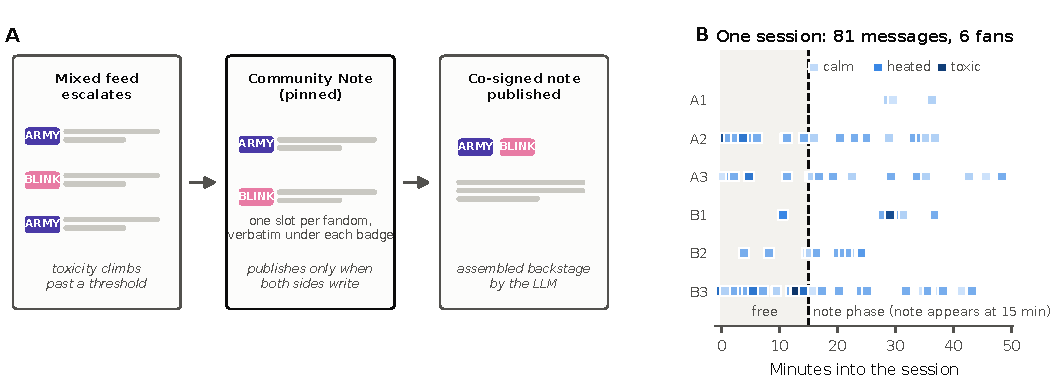
\includegraphics[width=\textwidth]{figures/fig_teaser}
  \caption{A ceasefire, not a peace treaty. (A)~When toxicity in a mixed
  ARMY--BLINK feed crosses a threshold, the platform pins a Community Note
  with one contribution slot per fandom; the note publishes only when both
  sides have written their part, each entry verbatim under its author's
  badge, assembled backstage by an LLM that never appears as a participant.
  (B)~One Day-1 session in both arms, one square per message, shaded from
  calm to toxic: six fans per arm (rows A1--A3 ARMY, B1--B3 BLINK) over
  \StatsessionMinutes{} minutes, with the assigned feature appearing at
  \StatnoteOnsetMin{} minutes (dashed line). In the Community Note arm
  (\StatshowExptN{} messages) the squares stay light after the line; in the
  control arm (\StatshowCtrlN{} messages) they darken. The session shown is
  the one with the median treatment effect of the five, not the strongest.}
  \Description{Left: a three-stage diagram showing an escalating mixed feed,
  a pinned Community Note with one slot for ARMY and one for BLINK, and a
  published co-signed note. Right: two timelines stacked, one per arm, each
  with six participant rows and one square per message shaded by toxicity,
  with a dashed line at 35 minutes marking the feature. In the Community
  Note arm the squares after the line are mostly light; in the control arm
  they are mostly dark.}
  \label{fig:teaser}
\end{teaserfigure}

\maketitle

\section{Introduction}

People like to fight online over who they are, not what to do. This hostility
toward out-groups, rooted in group identity rather than substantive
disagreement, is known as affective polarization~\cite{iyengar2012,
iyengar2019}, and it pervades online communities~\cite{rathje2021,
tornberg2022}. Common intuitive solutions target what people think. However,
neither works reliably: exposure to the other side can entrench
positions~\cite{bail2018}, and belief-correcting interventions produce
modest, short-lived effects~\cite{voelkel2023}. If the animosity is anchored
in identity, interventions aimed at information miss the layer where the
conflict lives.

Classic intergroup research suggests that hostility is reduced not by
changing beliefs, but by changing relationships between groups. When rival
groups become mutually dependent on a shared goal, cooperation fosters a
common identity and reduces conflict~\cite{sherif1954, gaertner2000}. This
mechanism, cooperative interdependence, has shown robust effects in
real-world settings~\cite{levine2005, mousa2020}. However, existing online
depolarization interventions target individuals rather than group
relationships~\cite{guess2023, combs2023, wojcik2022}, and none brings rival
groups into cooperative production. In this study, we investigate whether
structured co-creation between rival groups can reduce intergroup hostility
on online platforms.

Online fights are rarely intense from the first message. They accumulate: a
topic ignites them, and they burn only as long as the participants keep
feeding them attention. That dependence is the opening we exploit. We
instantiate the idea as Community Notes, a platform feature through which
members of rival groups co-author a single, publicly co-signed post---a task
that asks nothing of anyone's beliefs but takes a few minutes of everyone's
attention away from the fight. A pinned
prompt offers one slot per group; the note publishes only when both sides
have written their part, each entry verbatim under its author's badge.
Neither side can complete a note alone, and neither has to stop being itself.
The LLM behind the feature stays out of sight: it monitors the discussion and
publishes the finished note. Participants encounter a platform feature and
each other, not a machine.

Testing such a feature requires rival groups whose hostility is real,
identity-driven, and native to platforms. We chose K-pop fandom, one of the
largest transnational fan cultures online~\cite{jin2016, mclaren2020}, and
the rivalry between ARMY and BLINK, fandoms of BTS and BLACKPINK: it is
enduring, conducted almost entirely on platforms, and rests on no substantive
dispute, a near-pure case of identity-driven hostility~\cite{yin2020,
duffett2013}. We deploy the feature on KFeed, a Reddit-style forum built for
this research, where mixed sessions of ARMY and BLINK members discuss K-pop
topics with either the Community Note or an inert control feature. We
measure toxicity through automated scoring and human coding, and
qualitatively analyze how cross-group interaction changes. We ask:

\begin{itemize}
  \item \textbf{RQ1:} How do Community Notes affect polarized groups posting
  on online forums?
  \item \textbf{RQ2:} How does what they post change after the Community Note
  intervention?
\end{itemize}

In answering these questions, our work contributes: (1) a reusable platform
mechanism that operationalizes cooperative interdependence in an online
forum; (2) an extension of LLM-based depolarization from persuading
individuals to structuring how groups interact; and (3) empirical evidence
from real polarized communities that a shared task can call a ceasefire
without producing a peace: sessions with the note did not escalate while
matched control sessions did, the difference persisted a day later with no
feature on screen, and the calm came from the periphery of the fight rather
than its core.

\section{Related Work}

Defusing polarization in online forums raises three questions: what kind of
polarization it is, what reduces it, and what role an AI system can play. We
first characterize affective polarization as a group-level phenomenon rooted
in social identity. We then draw on cooperative interdependence theory to
elicit the requirements for our intervention. Finally, we examine how LLMs
have been used to intervene in online communities.

\subsection{Affective Polarization in Online Fan Communities}

Affective polarization refers to animosity toward an out-group that is rooted
in group membership rather than substantive
disagreement~\cite{iyengar2012, iyengar2019}. Social identity theory traces
this animosity to the self-concept: because people define themselves partly
through their groups, favoring the in-group and derogating the out-group
becomes a way of maintaining a positive self-image~\cite{tajfel1979}.
Strikingly, this requires almost nothing. In minimal group experiments,
assigning people to arbitrary, meaningless categories was enough to produce
discrimination between groups~\cite{tajfel1971}. Hostility follows from the
group boundary itself, not from any dispute across it. The intuitive remedy,
correcting what each side believes about the other, therefore addresses the
wrong layer. Polarization is a membership problem, not an information
problem.

Political contexts make this hard to see, because partisan identity is
entangled with real ideological stakes and the contribution of identity alone
cannot be isolated~\cite{mason2018}. Online fan communities present the
phenomenon in purer form. Rival fandoms sustain hostility toward one another
with no substantive dispute to resolve~\cite{duffett2013}. The bond runs
deeper than preference: fans incorporate their idol's successes and failures
into their own self-worth, basking in reflected glory when the idol
prevails~\cite{cialdini1976}, and the more strongly they identify, the less
able they are to distance themselves when the idol is
attacked~\cite{wann1990}.

This self-investment explains why fan conflict takes the form of costly,
active aggression rather than mere dislike. Among the most devoted fans,
personal and group identity can fuse, and fused individuals do not simply
favor their group: they act for it, willingly bearing personal costs to
defend it~\cite{swann2009, swann2012}. Notably, this conflict unfolds within
platform mechanics: fans fight with posts, downvotes, and coordinated
campaigns, in forums and comment sections, at times over the use of those
spaces themselves~\cite{yin2020, marwick2021}. Perceived threats to the
group's standing harden identification further rather than loosening
it~\cite{branscombe1999}. In idol and sports forums, toxicity and hostile
language accordingly concentrate around encounters with rival
groups~\cite{cleland2014, rathje2021}. K-pop fandoms are a prominent case,
organized, transnational, and highly active online~\cite{jin2016,
mclaren2020}.

HCI has largely overlooked this side of fandom: the field's fan research
centers on positive collective action~\cite{fiesler2016}, and fandom itself
remains a self-acknowledged gap~\cite{fiesler2016}. Fan communities thus
offer what political settings cannot: a near-pure case of identity-driven
animosity, unfolding entirely within platform mechanics, and a clean setting
for testing interventions that target identity rather than information.

\subsection{Cooperative Interdependence and Intergroup Contact}

The intuitive remedies for intergroup hostility are more contact and better
information. Neither reliably changes identity-based conflict. Exposing
partisans to opposing views entrenched their positions rather than softening
them~\cite{bail2018}, and a megastudy of depolarization interventions found
even the strongest effects modest and short-lived~\cite{voelkel2023}. Yet one
apparent failure reveals a design opportunity. In a field experiment, Iraqi
Christians were assigned to amateur soccer teams that were either
all-Christian or mixed with Muslim teammates~\cite{mousa2020}. Playing
together did not change their general attitudes toward Muslims, but it
changed their behavior. Months later, players from mixed teams were more
likely to train with Muslim peers and sign up for mixed leagues. Attitudes
rooted in identity are difficult to shift directly, while cooperative
behavior emerges when groups share a goal that neither side can achieve
alone.

This mechanism is known as cooperative interdependence. In the Robbers Cave
experiments, contact alone intensified competition between rival groups,
until they were placed in situations requiring collaboration toward
superordinate goals~\cite{sherif1954}. The Common Ingroup Identity Model
explains why. Working toward a shared outcome leads people to recategorize
themselves under a broader identity, extending the positive regard reserved
for the in-group to former out-group members~\cite{gaertner2000}. The
mechanism operates among real-world rivals. Manchester United fans who
encountered an injured jogger were more likely to help when he wore a United
shirt than a Liverpool one; when a shared identity as football fans had been
made salient beforehand, they helped the Liverpool supporter just as
readily~\cite{levine2005}. In both cases, behavior changed while group
identities stayed intact.

These findings set three requirements for interventions targeting
identity-driven conflict. Interaction must involve genuine interdependence,
since tasks that either group can complete alone provide no motivation for
recategorization~\cite{gaertner2000}. The shared identity must be layered on
top of existing subgroup identities rather than replacing them, because
attempts to erase group boundaries read as identity threats, which intensify
rather than reduce identification~\cite{branscombe1999, hornsey2000}. And the
shared identity must emerge from the interaction itself rather than being
imposed explicitly, because categorization follows the identities made
salient by the immediate situation~\cite{turner1987, levine2005}. Our
intervention is built to satisfy all three.

Online platforms are deeply involved in shaping these interactions. Platform
affordances enable rival communities to organize, amplify, and sustain
hostility at scale~\cite{marwick2021}, and platform design can further
intensify rivalry among fandoms~\cite{yin2020}. But the same mechanisms that
structure conflict can be redesigned to support cooperation. Existing
approaches intervene at three points, setting aside moderation, which
suppresses hostile expression without changing the relationship between
groups. Exposure-based designs modify what users encounter across group
boundaries, such as cross-cutting feeds or shared casual
games~\cite{bail2018, guess2023}. Matching-based designs modify who interacts
with whom, pairing individuals across the divide~\cite{combs2023}.
Correction-based designs modify how contested information is evaluated, most
notably Community Notes, where a bridging mechanism surfaces contributions
considered helpful by users with otherwise opposing
viewpoints~\cite{wojcik2022}.

These approaches leave the relationship between the groups unchanged.
Polarized communities remain audiences exposed to one another, strangers
temporarily paired, or adversaries evaluating each other's claims. None
intervenes at the point where relationships are formed through joint
creation, where opposing groups must produce something together rather than
merely encounter, discuss, or judge one another. Cooperative interdependence,
the mechanism with the strongest field evidence for changing intergroup
behavior, has never been built into a platform and tested with members of
real polarized communities.

\subsection{LLM Interventions in Online Communities}

When AI systems intervene in online conflict, they take one of the roles that
conflict resolution research assigns to human third parties. Moderators
enforce conduct rules after violations occur, facilitators manage
participation without touching content, and mediators contribute questions
and proposals of their own~\cite{moore2014}. LLMs have now filled each seat.
They moderate at scale~\cite{gilardi2023}, suggest real-time rephrasings that
make contentious conversations feel heard~\cite{argyle2023}, reduce belief in
conspiracy theories through persuasive dialogue~\cite{costello2024}, and
mediate live debates with psychologically grounded
strategies~\cite{tessler2024}. Across this spectrum, what varies is how much
the system contributes to the conversation.

Two features hold constant. First, the intervention targets individual minds.
Each system persuades, corrects, or calms particular interlocutors, treating
polarization as something wrong in what a person thinks. The results echo a
familiar pattern. LLM dialogue can move issue positions, yet affective
polarization stays where it was~\cite{costello2024, tessler2024}, the same
dissociation Mousa observed on the soccer field, and the one expected if
hostility follows membership rather than belief. Second, the system is a
visible party to the exchange. Users know they are talking with, or being
coached by, a machine, and disclosed AI authorship invites discounting and
reactance~\cite{jakesch2019}. The deeper problem is theoretical. An agent
that openly steers people toward common ground is doing precisely what the
third requirement rules out, announcing a shared identity rather than letting
the situation produce one.

Across this spectrum, then, the LLM holds a seat in the interaction, and
users are acted upon by the machine. No existing work inverts that
allocation, returning the interaction entirely to the users while confining
the system to the conditions under which they meet. In that position the LLM
shapes when cooperation becomes possible and how a joint product takes form,
but what participants encounter, throughout, is each other.

Together, the three literatures leave a single gap. Affective polarization
has been studied almost entirely in political settings, leaving its purest
identity-driven form in fan communities unexamined~\cite{fiesler2016,
duffett2013}. Cooperative interdependence, the mechanism with the strongest
field evidence, has never been built into a platform~\cite{sherif1954,
mousa2020}. And LLM interventions have varied the system's role within the
conversation without asking whether it belongs in the conversation at
all~\cite{argyle2023, tessler2024}. Our work sits at this intersection. We
build a community notes feature through which members of rival fandoms
co-author a single, publicly co-signed post, with the LLM working only
backstage, and test it with two polarized communities on a live forum.

\section{Experiment: Community Notes in a Polarized Forum}

We conducted a two-day experiment to test whether a co-authorship feature
reduces toxicity between rival fandoms. Participants, self-identified members
of ARMY or BLINK, joined mixed sessions of ARMY and BLINK members on KFeed, a
Reddit-style forum built for this research, and discussed K-pop topics under
their fandom badge. Discussion threads were seeded with prompts, including
toxic arguments drawn from pilot sessions, so that hostile, neutral, or
constructive interaction could emerge naturally.

Throughout each session, the platform scored incoming posts for toxicity in
real time. When session-level toxicity crossed a threshold determined from
pilot sessions, the assigned feature appeared in the feed; in the sessions
reported here this happened \StatnoteOnsetMin{} minutes into every Day-1
session in both arms, by which point toxicity had climbed past the threshold
in each. \todonote{confirm whether the trigger was threshold-driven or fixed
at the 35-minute mark in the deployed protocol, and say which.} We randomly
assigned sessions to two conditions:

\begin{enumerate}
  \item \textbf{Community Notes treatment:} the feature that appeared was a
  Community Note, a pinned prompt framed at the K-pop level with one
  contribution slot per fandom. The note published only when both sides had
  written their part, each entry preserved verbatim under its author's badge.
  \item \textbf{Inert feature control:} the feature that appeared was matched
  to Community Notes on visual salience and interaction cost but required no
  cross-fandom contribution. \todonote{describe the inert feature as
  fielded.} Following the placebo-activity logic of Combs et
  al.~\cite{combs2023}, this condition ensures that both arms experience a
  triggered platform event, so that novelty and regression toward the mean
  are shared across conditions and the treatment effect is identified by the
  condition-by-phase contrast.
\end{enumerate}

On Day 2, participants returned to the same session composition and discussed
without any feature, allowing us to examine whether behavioral changes
persisted after the mechanism was removed.

\subsection{Building KFeed and the Community Notes Feature}

KFeed supports community feeds, threaded discussion, moderator-pinned posts,
and persistent fandom badges on every post. The Community Notes feature
translates the three requirements from Section~2.2 into interface rules
(Figure~\ref{fig:teaser}A).

\begin{itemize}
  \item \textbf{A note needs both fandoms.} After one side submits, the entry
  sits waiting under its author's badge until a rival answers. Neither side
  can write for the other or publish alone.
  \item \textbf{Both badges stay visible.} From draft to publication, each
  entry carries its author's fandom badge, and votes accrue to the note as a
  whole rather than to either half.
  \item \textbf{Nothing is said about shared identity.} Prompts address K-pop
  fans at large, but no instruction tells participants to identify as one
  group, and entries are published verbatim rather than merged.
\end{itemize}

\subsection{Configuring the Backstage LLM}

An LLM performs two functions in the system, both invisible to participants.
First, it monitors the discussion: incoming posts are scored for toxicity in
real time, producing the session-level signal that triggers the assigned
feature. Second, it publishes the Community Note: once both fandom slots are
filled, it verifies that the note contains one entry per fandom and assembles
the two entries verbatim into the pinned format. The model does not write or
rewrite anyone's words, does not converse with participants, and claims no
identity. We keep it backstage deliberately: an agent that visibly steered
rivals toward common ground would announce the shared identity that the
design requires the situation to produce. In our system, the LLM decides when
the cooperative task appears and makes its outcome public; the cooperation
itself belongs entirely to the participants.

\subsection{Recruitment and Participants}

We recruited participants through fandom communities on social platforms,
screening with an open-ended fandom identification question to avoid
signaling the study's focus, with working language and location as
eligibility criteria. \StatnParticipants{} participants took part in the
sessions reported here, \StatnPerSession{} per session and arm (three ARMY
and three BLINK), each attending both days; no participant appeared in more
than one session.

\subsection{Procedure}

Participants completed a pre-survey at recruitment (fandom identification,
trait covariates, and eligibility screening), then joined fixed time slots
and confirmed readiness before each session. Sessions lasted approximately
one hour per day on two consecutive days. A survey followed each day's
session: after Day 1, the outcome battery; after Day 2, the outcome battery
again, feature-specific items, and a funneled suspicion probe. After the Day
2 survey, we invited a subset of participants to semi-structured interviews
about their experience across both days, sampling from both fandoms and both
conditions.

\subsection{Measures}

Toxicity is the primary outcome, scored on pre-moderation text by Perspective
API~\cite{lees2022} and independent human coding following Coe, Kenski, and
Rains's incivility codebook~\cite{coe2014}, supplemented by a K-pop
incivility lexicon validated before use with inter-rater reliability
reported. The platform stores the result as a 0--100 score per message, which
we report on that scale. \todonote{state how the platform's 0--100 score is
composed: which Perspective attributes, how they are weighted, and how the
human codes and lexicon enter the final score.} Each message in the export
additionally carries three codes applied by the research team: whether it
refers to the rival fandom and, if so, whether as ``they'' or by name;
whether it addresses the note task rather than the thread it was posted in;
and a flag marking the heaviest poster of each session and arm.
\todonote{report who applied the message codes and their inter-rater
reliability.} Survey outcomes adapt validated instruments to the fandom
boundary, following the battery of Rajadesingan et
al.~\cite{rajadesingan2020}: the feeling thermometer toward rival-fandom
members~\cite{iyengar2012}, common in-group identity representation as the
mediator~\cite{gaertner2000}, and fandom identification via a fan
identification scale~\cite{wann1993}, which also tests that the intervention
does not erode subgroup identity. Behavioral logs capture cross-fandom
references and pronoun use~\cite{pennebaker2011}. Reactance serves as a
backfire guardrail~\cite{brehm1966}.

\subsection{Analysis}

For RQ1, we compare toxicity across conditions and phases. Because both
conditions are triggered at the same point, the treatment effect is
identified by the condition-by-phase contrast rather than by a before--after
comparison: we report it as a difference-in-differences over sessions (the
control arm's change from before to after the feature minus the note arm's,
one value per session, tested against zero) and, at the message level, as
the condition-by-phase interaction in a linear model. The session is the
unit of inference throughout; participant- and message-level tests are
reported alongside for the reader's calibration, not as independent
evidence. Day 2 tests whether changes persist. For RQ2, we use the message
codes (rival-fandom references, pronouns, and note-task topic) and two
researchers will code forum posts and interview transcripts for shifts in
cross-group interaction.

\section{Results}

We report \StatnSessions{} two-day sessions, each run in both arms with a
fresh mixed group of \StatnPerSession{} ARMY and BLINK members, for
\StatnParticipants{} participants and \StatnMessages{} messages
(\StatnDayOneMsgs{} on Day 1, \StatnDayTwoMsgs{} on Day 2; between
\StatminSessionMsgs{} and \StatmaxSessionMsgs{} messages per session and
arm on Day 1). On Day 1 the assigned feature appeared \StatnoteOnsetMin{}
minutes into each session; on Day 2 the same participants discussed without
it. Survey results draw on the \StatsurveyN{} treatment-arm participants of
the pilot cohorts (\StatsurveyCohorts) who completed the post-session
battery, none of whom was removed by our two pre-registered screens
(straightlining across the battery: \StatnStraightlinedExpt{} excluded;
rating the session as not heated, our manipulation check: \StatnFailedHeat{}
excluded, minimum rating \StatminHeat/5). \todonote{the battery for the five
sessions reported here has not been exported; the survey figures below are
from the pilot cohorts and must be replaced or explicitly labelled as pilot
data.} Table~\ref{tab:phases} summarizes Day 1 by arm and phase.

\begin{table}
  \caption{Day 1 by arm and phase: the first \StatnoteOnsetMin{} minutes
  (before the feature) against the remainder (after). The arms are alike
  before the feature; afterwards the control arm escalates and the note arm
  does not.}
  \label{tab:phases}
  \begin{tabular}{lcccc}
    \toprule
    & \multicolumn{2}{c}{Community Note arm} & \multicolumn{2}{c}{Control arm} \\
    \cmidrule(lr){2-3} \cmidrule(lr){4-5}
    & Before & After & Before & After \\
    \midrule
    Messages & \StatexptPreN & \StatexptPostN & \StatctrlPreN & \StatctrlPostN \\
    Mean toxicity (SD) & \StatexptPreM{} (\StatexptPreSD) & \StatexptPostM{} (\StatexptPostSD) & \StatctrlPreM{} (\StatctrlPreSD) & \StatctrlPostM{} (\StatctrlPostSD) \\
    Messages scoring $\geq 60$ & \StatexptPreHighPct\% & \StatexptPostHighPct\% & \StatctrlPreHighPct\% & \StatctrlPostHighPct\% \\
    Messages per minute & \StatexptRatePre & \StatexptRatePost & \StatctrlRatePre & \StatctrlRatePost \\
    Rival fandom as ``they'' (per message) & \StatexptTheyPre & \StatexptTheyPost & \StatctrlTheyPre & \StatctrlTheyPost \\
    Rival fandom by name (per message) & \StatexptNamedPre & \StatexptNamedPost & \StatctrlNamedPre & \StatctrlNamedPost \\
    Messages about the note task & \StatexptTaskPreN & \StatexptTaskPct\% & \StatctrlTaskPreN & \StatctrlTaskPct\% \\
    \bottomrule
  \end{tabular}
\end{table}

\subsection{The Note Prevented the Escalation the Control Arm Shows (RQ1)}

\subsubsection{Both arms were alike, and climbing, before the feature.}
In the \StatnoteOnsetMin{} minutes before the feature the two arms were
indistinguishable: mean message toxicity was \StatexptPreM{} in the note arm
and \StatctrlPreM{} in the control arm (Welch
$t(\StatpreArmDf)=\StatpreArmT$, $p=\StatpreArmP$; session-paired
$t(\StatdidDf)=\StatprePairT$, $p=\StatprePairP$). Neither arm was calm:
toxicity rose by about a point a minute in both (note arm slope
\StatexptPreSlope{} per minute, control \StatctrlPreSlope, both
$p<.001$), from around \StatexptWinFirst{} in the first five-minute window
to \StatexptWinPreMax{} and \StatctrlWinPreMax{} in the window just before
the feature (Figure~\ref{fig:windows}). The trigger fired, in other words,
into a fight that was still heating up.

\subsubsection{After the feature, the control arm escalated and the note arm did not.}
In the control arm, toxicity rose from \StatctrlPreM{} before the inert
feature to \StatctrlPostM{} after it (Welch
$t(\StatctrlPrePostDf)=\StatctrlPrePostT$, $p\StatctrlPrePostP$), and it
rose in every session, by between \StatctrlChangeMin{} and
\StatctrlChangeMax{} points. In the note arm it went from \StatexptPreM{} to
\StatexptPostM{} ($t(\StatexptPrePostDf)=\StatexptPrePostT$,
$p=\StatexptPrePostP$), with session changes between \StatexptChangeMin{}
and \StatexptChangeMax{} points. The treatment effect is the difference
between these two changes: \StatdidM{} points over sessions (SD
\StatdidSD, range \StatdidMin{} to \StatdidMax;
$t(\StatdidDf)=\StatdidT$, $p\StatdidP$), and in the message-level model
a condition-by-phase interaction of \StatolsIntB{} points (SE
\StatolsIntSE, $t(\StatolsDf)=\StatolsIntT$, $p\StatolsIntP$). Leaving
out any one session moves the difference only between \StatlooMin{} and
\StatlooMax{} points. Figure~\ref{fig:participants} shows the four means
with every participant behind them.

\begin{figure*}
  \centering
  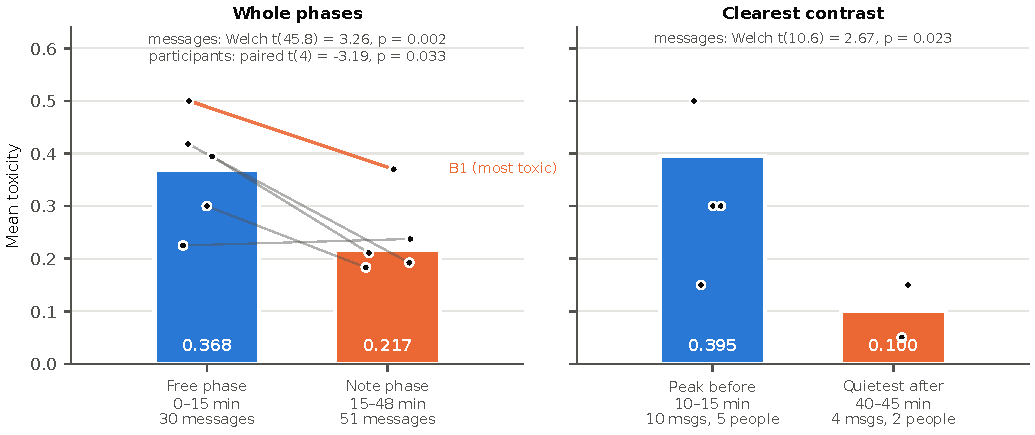
\includegraphics[width=\textwidth]{figures/fig_participants}
  \caption{The escalation the note prevented, with both the averages and
  the people behind them. Left: Day-1 mean toxicity before and after the
  feature in each arm (bars: message-level means; dots: participants,
  connected across the two phases; thick lines: the heaviest poster of each
  session). Right: each participant's change from before to after,
  split into the platform-coded heaviest poster of each session and
  everyone else. In the note arm the periphery cooled while the core heated;
  in the control arm both rose together.}
  \Description{Left: four bars with participant dots. Community Note arm:
  45.9 before, 44.2 after, with most participant lines falling and five
  thick lines rising. Control arm: 46.9 before, 68.8 after, with almost
  every line rising. Right: four bars of mean change. Community Note arm:
  periphery minus 18.2 with 24 dots mostly below zero, heaviest posters
  plus 14.1 with all five dots above zero. Control arm: periphery plus 21.4
  and heaviest posters plus 23.3, both with dots above zero.}
  \label{fig:participants}
\end{figure*}

The result does not depend on who is counted (Table~\ref{tab:robust}).
Restricting the analysis to participants who posted at least six or at
least ten messages leaves the difference-in-differences between
\StatrobTenDid{} and \StatrobSixDid{} points; excluding the heaviest poster
of each session raises it to \StatrobPeriDid{} points, for a reason the
next section explains.

\begin{table}
  \caption{The condition-by-phase difference survives restricting the
  sample. Session-level means before and after the feature by arm, and the
  difference-in-differences (control change minus note-arm change) tested
  over the five sessions.}
  \label{tab:robust}
  \begin{tabular}{lccccc}
    \toprule
    & & \multicolumn{1}{c}{Note arm} & \multicolumn{1}{c}{Control arm} & \multicolumn{2}{c}{Difference-in-differences} \\
    \cmidrule(lr){3-3} \cmidrule(lr){4-4} \cmidrule(lr){5-6}
    Participants included & $n$ & before $\to$ after & before $\to$ after & points & $t(\StatdidDf)$ ($p$) \\
    \midrule
    All & \StatrobAllPart & \StatrobAllExptPre{} $\to$ \StatrobAllExptPost & \StatrobAllCtrlPre{} $\to$ \StatrobAllCtrlPost & \StatrobAllDid & \StatrobAllDidT{} (\StatrobAllDidP) \\
    $\geq 6$ messages & \StatrobSixPart & \StatrobSixExptPre{} $\to$ \StatrobSixExptPost & \StatrobSixCtrlPre{} $\to$ \StatrobSixCtrlPost & \StatrobSixDid & \StatrobSixDidT{} (\StatrobSixDidP) \\
    $\geq 10$ messages & \StatrobTenPart & \StatrobTenExptPre{} $\to$ \StatrobTenExptPost & \StatrobTenCtrlPre{} $\to$ \StatrobTenCtrlPost & \StatrobTenDid & \StatrobTenDidT{} (\StatrobTenDidP) \\
    Heaviest poster excluded & \StatrobPeriPart & \StatrobPeriExptPre{} $\to$ \StatrobPeriExptPost & \StatrobPeriCtrlPre{} $\to$ \StatrobPeriCtrlPost & \StatrobPeriDid & \StatrobPeriDidT{} (\StatrobPeriDidP) \\
    \bottomrule
  \end{tabular}
\end{table}

\subsubsection{The note did not end the discussion.}
Messages kept arriving in the note arm at \StatexptRatePost{} per minute
after the feature against \StatexptRatePre{} before it (rate ratio
\StatexptRateRatio, exact test of equal rates $p=\StatexptRateP$), the
same as in the control arm (\StatctrlRatePre{} to \StatctrlRatePost).
\StatexptKeptPosting{} of the \StatnPerArm{} note-arm participants posted in
both phases, and the one who had been silent before the note joined in after
it. The ceasefire cooled the exchange without emptying the room.

\subsection{The Periphery Cooled and the Core Heated (RQ1)}

\subsubsection{The flat arm mean hides two opposite movements.}
At the participant level, the note arm did fall: for the \StatexptPairN{}
participants who posted in both phases, mean toxicity went from
\StatexptPrePartM{} to \StatexptPostPartM{}, a within-participant change of
\StatexptPairDiff{} points (paired $t(\StatexptPairDf)=\StatexptPairT$,
$p\StatexptPairP$, $d_z=\StatexptPairDz$), and \StatexptNDeclined{} of the
\StatexptPairN{} became less toxic. In the control arm the change was
\StatctrlPairDiff{} points ($t(\StatctrlPairDf)=\StatctrlPairT$,
$p\StatctrlPairP$, $d_z=\StatctrlPairDz$), and \StatctrlNRose{} of
\StatctrlPairN{} became more toxic. The participant-level decline in the
note arm is larger than its message-level one because the participants who
rose wrote more of the messages.

Those participants were the core of the fight. The platform flags the
heaviest poster of each session and arm; these \StatheavyTotalN{} people
wrote \StatheavyMsgPct\% of all Day-1 messages, and \StatheavyBlinkN{} of
the \StatheavyTotalN{} were BLINK. In the note arm, all five heavy posters
became \emph{more} toxic after the note, from \StatexptHeavyPreM{} to
\StatexptHeavyPostM{} on average (changes of \StatexptHeavyDiffMin{} to
\StatexptHeavyDiffMax{} points), while the other \StatexptPeriN{}
participants went from \StatexptPeriPreM{} to \StatexptPeriPostM{}
(\StatexptPeriNDeclined{} of \StatexptPeriN{} declined; core versus
periphery, Welch $t(\StatexptHeavyPeriDf)=\StatexptHeavyPeriT$,
$p\StatexptHeavyPeriP$). The heavy posters' share of the arm's messages
also rose, from \StatexptHeavySharePre\% to \StatexptHeavySharePost\%. In
the control arm core and periphery moved together (\StatexptHeavyDiff{}
versus \StatexptPeriDiff{} points in the note arm; \StatctrlHeavyDiff{}
versus \StatctrlPeriDiff{} in the control arm, $p=\StatctrlHeavyPeriP$;
Figure~\ref{fig:participants}, right). The note did not lower everyone. It
split the room.

\subsubsection{The distributions show the split.}
Figure~\ref{fig:histogram} shows the message-level distributions. Before the
feature the two arms overlap. Afterwards the control arm's distribution
moves as a block to the right: \StatctrlPostHighPct\% of its messages score
60 or above, against \StatctrlPreHighPct\% before. The note arm's
distribution instead spreads out, its standard deviation rising from
\StatexptPreSD{} to \StatexptPostSD: most of its mass moves left, and a
smaller mass, the heavy posters' messages, moves right, leaving
\StatexptPostHighPct\% of messages at 60 or above.

\begin{figure*}
  \centering
  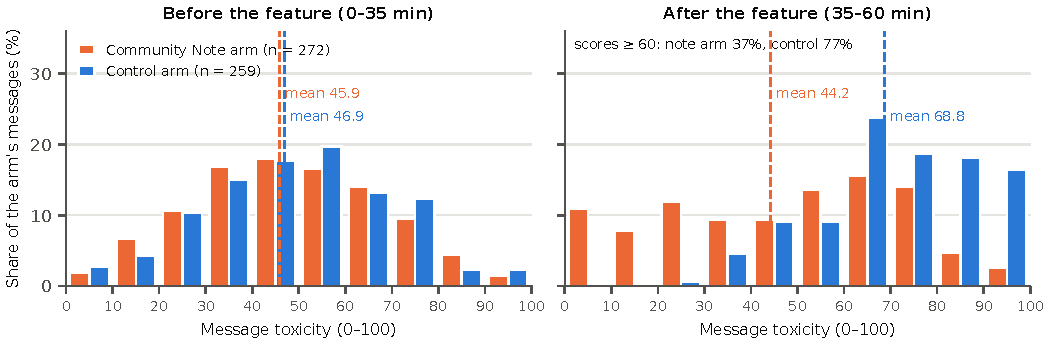
\includegraphics[width=\textwidth]{figures/fig_histogram}
  \caption{Distribution of message toxicity before and after the feature,
  by arm (share of each arm's messages per 10-point bin). Before the
  feature the arms overlap. Afterwards the control distribution moves as a
  block to the right, while the note arm's spreads: its bulk moves left and
  a smaller mass, the heavy posters, moves right.}
  \Description{Two paired histograms. Before the feature, orange (note arm)
  and blue (control) bars follow the same hump centred near 45. After the
  feature, blue bars pile up between 60 and 100 with a mean of 68.8, while
  orange bars spread across the whole range with a mean of 44.2, with mass
  both at 0 to 30 and at 60 to 80.}
  \label{fig:histogram}
\end{figure*}

\subsection{The Conversation Moved to the Task (RQ2)}

\subsubsection{A third of the note arm's messages were about the note.}
After the feature, \StatexptTaskPct\% of the note arm's messages
(\StatexptTaskN{} of \StatexptPostN) addressed the note task rather than
the thread they were posted in, against \StatctrlTaskPct\% in the control
arm (\StatctrlTaskN{} of \StatctrlPostN; Fisher's exact $p\StattaskFisherP$).
Those task messages were calmer than the rest (\StatexptTaskTox{} versus
\StatexptOrigTox; Welch $t(\StatexptTaskOrigDf)=\StatexptTaskOrigT$,
$p=\StatexptTaskOrigP$), but the more telling number is the other one: the
note arm's messages that stayed on the original threads averaged
\StatexptOrigTox, only \StatexptOrigPreDiff{} points above the arm's
pre-feature mean, where the control arm's rose to \StatctrlPostM. The note
did not just siphon off calm messages; the fight it left behind did not
heat up either.

\subsubsection{They became names.}
References to the rival fandom as ``they'' fell by \StatexptTheyDropPct\%
in the note arm, from \StatexptTheyPre{} to \StatexptTheyPost{} per message
(Fisher's exact $p\StatexptTheyFisherP$), while references to the rival
fandom by name rose from \StatexptNamedPre{} to \StatexptNamedPost. The
share of messages referring to the rival fandom at all barely moved
(\StatexptOutPre{} to \StatexptOutPost). In the control arm ``they'' stayed
where it was (\StatctrlTheyPre{} to \StatctrlTheyPost, $p=\StatctrlTheyFisherP$)
and so did naming (\StatctrlNamedPre{} to \StatctrlNamedPost). Participants
in the note arm kept talking about the other side about as often; what
changed is that they named it instead of pointing at it.

\subsubsection{Conflict moved from works to persons to identity.}
Focus-group participants described a similar escalation pattern across
discussions. Conflicts often began with disagreements about works, such as
comebacks, album sales, view and like counts on YouTube, or choreography.
They then shifted to comments about the idol, followed by comments about the
other participant, and finally to broader statements about fandom identity:
\textit{``\ldots when they [BLINKs] talk about BTS, they would say that oh,
we ARMY have a fetish of ugly men. They would say we have a problem with
aesthetics.''} (P\#, focus group). \todonote{replace P\# with the participant
code.} Participants described the note's interruption as briefly taking them
out of the argument, a state one described as \textit{tuozhan}, or standing
down: not agreement, but stepping away from that particular fight.
\todonote{add supporting quote from transcript.}

Together, these results show that the conversation changed at the same time
as the escalation stopped. We do not claim that the topic shift caused it.

\subsection{The Ceasefire Minute by Minute}

Figure~\ref{fig:windows} shows both days in \StatwindowMin-minute windows,
pooled over the five sessions with each session drawn faintly behind. On
Day 1 the two arms climb together for \StatnPreWindows{} windows. At the
feature they part: the control arm continues to \StatctrlWinFirstPost{} in
the first window after the feature and \StatctrlWinLast{} in the last,
while the note arm drops to \StatexptWinFirstPost{} and then
\StatexptWinPostMin{} (\StatexptWinPostMinLabel{} minutes), half of the
\StatexptWinPreMax{} it had reached in the window before the note (Welch
$t(\StatpeakTroughDf)=\StatpeakTroughT$, $p\StatpeakTroughP$; we report
this peak-to-trough contrast as descriptive, since its windows are chosen
after the fact; the control arm reads \StatctrlAtPeakWin{} and
\StatctrlAtTroughWin{} in the same two windows). The note arm then drifts
back up over the remaining windows (\StatexptWinPostMax{} in the last;
post-feature slope \StatexptPostSlope{} per minute, $p=\StatexptPostSlopeP$),
so that by the end of Day 1 the gap between the arms had narrowed to
\StatlastWinGap{} points. Within the hour, the pause was decaying.

\begin{figure*}
  \centering
  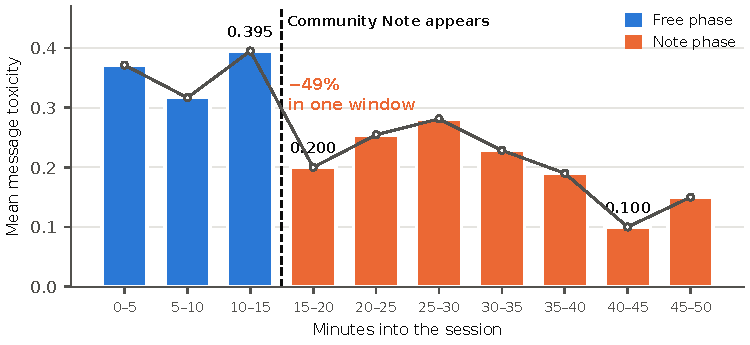
\includegraphics[width=\textwidth]{figures/fig_windows}
  \caption{Mean toxicity in \StatwindowMin-minute windows (bold: five
  sessions pooled; faint: each session). Day 1: both arms climb for
  \StatnoteOnsetMin{} minutes; at the feature the control arm keeps
  climbing and the note arm drops, then drifts back. Day 2, no feature: the
  note arm starts near its Day-1 baseline and never climbs; the control arm
  starts where it left off. Messages per window, note arm: \StatexptWinNs;
  control arm: \StatctrlWinNs.}
  \Description{Two line charts. Day 1: orange (note arm) and blue (control)
  lines rise together from about 30 to about 65 by minute 35, marked by a
  dashed line; after it the blue line continues to 61, 73, 68, 70 and 76
  while the orange line falls to 47 and 32, then rises to 36, 45 and 58.
  Day 2: the blue line runs between 67 and 76 from the first window; the
  orange line runs between 38 and 52.}
  \label{fig:windows}
\end{figure*}

\subsection{The Ceasefire Held on Day 2}

On Day 2 the same participants returned and discussed without any feature.
The note arm's sessions averaged \StatexptDayTwoSessM{} (range
\StatexptDayTwoSessMin{} to \StatexptDayTwoSessMax), no different from
their Day-1 post-feature level (\StatexptPostSessM; paired
$t(\StatdidDf)=\StatexptPostDayTwoT$, $p=\StatexptPostDayTwoP$) or from
their Day-1 level before the feature (\StatexptPreSessM;
$t(\StatdidDf)=\StatexptPreDayTwoT$, $p=\StatexptPreDayTwoP$). The control
arm's sessions averaged \StatctrlDayTwoSessM{} (range
\StatctrlDayTwoSessMin{} to \StatctrlDayTwoSessMax), no different from
their Day-1 post-feature level (\StatctrlPostSessM;
$t(\StatdidDf)=\StatctrlPostDayTwoT$, $p=\StatctrlPostDayTwoP$) and far
above their Day-1 pre-feature level ($t(\StatdidDf)=\StatctrlPreDayTwoT$,
$p\StatctrlPreDayTwoP$). Across arms, every note-arm session was calmer on
Day 2 than its paired control session, by \StatdayTwoGapMin{} to
\StatdayTwoGapMax{} points (mean \StatdayTwoGap; paired
$t(\StatdidDf)=\StatdaytwoPairT$, $p\StatdaytwoPairP$; message-level Welch
$t(\StatdaytwoArmDf)=\StatdaytwoArmT$; Figure~\ref{fig:days}).

Neither arm re-ran Day 1's climb. The control arm started Day 2 at
\StatctrlDayTwoWinFirst{} in its first five-minute window, where it had
ended Day 1, and never fell below \StatctrlDayTwoWinMin. The note arm
started at \StatexptDayTwoWinFirst, where it had started Day 1, and never
rose above \StatexptDayTwoWinMax{} (Figure~\ref{fig:windows}, right). The
pronoun pattern carried over too: on Day 2, ``they'' references ran at
\StatexptTheyDayTwo{} per message in the note arm against
\StatctrlTheyDayTwo{} in the control arm. Each arm resumed at the level it
had reached the day before, and the note arm had never reached one.

\begin{figure}
  \centering
  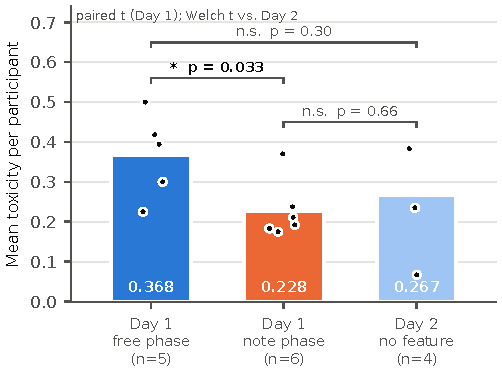
\includegraphics[width=0.8\linewidth]{figures/fig_days}
  \caption{Session-level mean toxicity in the Day-1 phase before the
  feature, the Day-1 phase after it, and Day 2 without any feature, by arm
  (bars: mean of the five sessions; dots: sessions, connected). Within each
  arm, Day 2 does not differ from the Day-1 post-feature phase (paired $t$
  over sessions); across arms, every note-arm session is calmer than its
  paired control session on Day 2.}
  \Description{Six bars with session dots. Community Note arm: 46.1 before,
  43.8 after, 44.5 on Day 2, with a bracket marked not significant, p =
  0.78, between the last two. Control arm: 45.8 before, 68.8 after, 71.6 on
  Day 2, with a bracket marked not significant, p = 0.17. A bracket across
  the two Day 2 bars is marked three stars, p = 0.0008.}
  \label{fig:days}
\end{figure}

\subsection{Attitudes Did Not Change (Pilot Survey)}

The post-session battery available to us comes from the treatment-arm
participants of the \StatsurveyNCohorts{} pilot cohorts ($n=\StatsurveyN$),
not from the five sessions above, so we read it as a description of how
participants receive the note rather than as an outcome of these sessions.
Participants rated the note low in legitimacy (\StatlegitM/5) and high in
reactance (\StatreactM/5). Perceived similarity to the rival fandom was near
the scale midpoint (\StatsimilM/5), while the thermometer gap between their
own and the rival fandom was \StatthermGap{} points
(Table~\ref{tab:survey}). These ratings suggest that participants did not
respond to the note because they accepted its authority or felt more
positively toward the rival fandom.

The hostility, however, stops at the screen. On the same battery, the item
participants endorsed most strongly was that a member of the rival fandom
could be a friend in real life (\StatcontactFriends/5), the only item above
the scale midpoint, while they rated rival fans as unintelligent and immoral
(\StatpercM/5) and kept them 60 thermometer points below their own fandom
(Figure~\ref{fig:attitudes}). Contact intentions as a whole sat exactly at
the midpoint ($t(9)=\StatcontactVsMidT$, $p=\StatcontactVsMidP$ against
neutral). The superordinate identity the note addressed was available to
them: they rated K-pop fans as a whole at \StatthermKpop, warmer than their
own fandom, while every similarity item toward the rival fandom sat at the
midpoint (general \StatsimilGeneral, interests \StatsimilInterests, values
\StatsimilValues, caring about the same things \StatsimilCare): the same kind
of fan, of a different idol. \todonote{entry-of-day survey export pending:
add before/after change in the thermometer gap, the K-pop thermometer and
the contact items, and the two feature items (note changes the atmosphere;
fandom still matters).} The enemy in the thread, in other words, is not an enemy in the
room---a distinction participants also drew unprompted in the focus groups.
\todonote{add the focus-group quote on online versus real-life enemies.}

\begin{figure*}
  \centering
  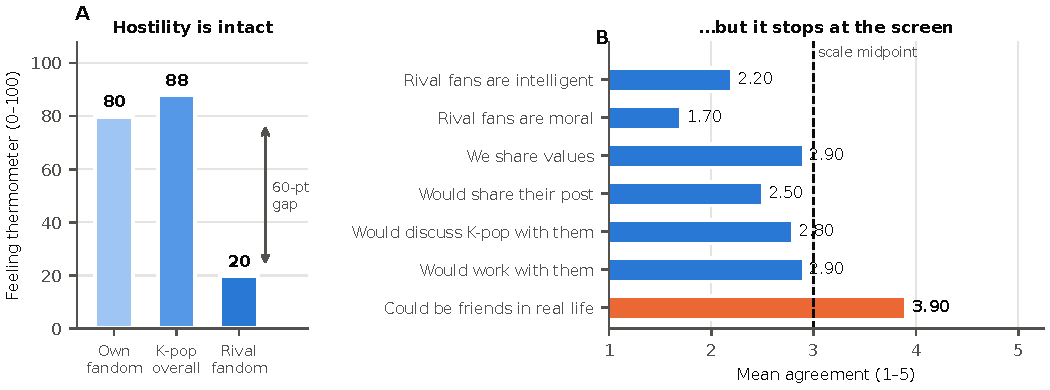
\includegraphics[width=\textwidth]{figures/fig_attitudes}
  \caption{The ceasefire did not make them like each other, but the dislike
  is confined to the platform (pilot cohorts, $n=\StatsurveyN$). (A)~Feeling
  thermometer toward one's own fandom, K-pop fans overall, and the rival
  fandom: the shared identity is warm, the rival is cold. (B)~Agreement
  items about rival-fandom members on a 1--5 scale: they are rated as
  unintelligent and immoral, yet the single item participants endorsed most
  was that a rival fan could be a friend in real life.}
  \Description{Left: three bars on a 0 to 100 thermometer, own fandom 80,
  K-pop overall 88, and rival fandom 20, with the 60-point own-rival gap
  marked. Right: horizontal bars for
  seven agreement items on a 1 to 5 scale; rival fans are intelligent 2.20,
  rival fans are moral 1.70, we share values 2.90, would share their post
  2.50, would discuss K-pop with them 2.80, would work with them 2.90, and
  could be friends in real life 3.90, the only bar past the midpoint line at
  3, highlighted.}
  \label{fig:attitudes}
\end{figure*}

Survey responses and focus-group accounts pointed in different directions.
While participants rated the note low in legitimacy, they described the
pop-out itself as a useful feature: \textit{``This function\ldots{} well I
don't need to think about blinks too much. I just wrote my own opinion on the
note and that's it. But at least it is useful because I\ldots''} (P\#, focus
group). \todonote{quote is cut off; complete from transcript and replace P\#
with the participant code.}

\begin{table}
  \caption{Post-session survey outcomes for treatment-arm participants of
  the pilot cohorts ($n=\StatsurveyN$). Scale items are 1--5; thermometers
  are 0--100. Participants experienced the sessions as heated, granted the
  note little legitimacy, reported high reactance, and their outgroup
  attitudes stayed cold.}
  \label{tab:survey}
  \begin{tabular}{lc}
    \toprule
    Measure & M (SD) \\
    \midrule
    Legitimacy of the note & \StatlegitM{} (\StatlegitSD) \\
    Reactance toward the note & \StatreactM{} (\StatreactSD) \\
    Perceived similarity to rival fandom & \StatsimilM{} (\StatsimilSD) \\
    Perception of rival fandom (intelligent, moral) & \StatpercM{} (\StatpercSD) \\
    Cross-fandom contact intentions & \StatcontactM{} (\StatcontactSD) \\
    Session felt heated / attacked & \StatsessM{} (\StatsessSD) \\
    Thermometer: own fandom & \StatthermOwn \\
    Thermometer: rival fandom & \StatthermRival \\
    Thermometer gap (own $-$ rival) & \StatthermGap{} (\StatthermGapSD) \\
    \bottomrule
  \end{tabular}
\end{table}

\section{Discussion}

\subsection{A Shared Task Without a Shared Identity}

The CIIM framework was necessary, but it worked differently from how we
expected. It did not produce a common identity. It produced a shared task
that both sides were willing to enter for a short time.

We built the feature to satisfy three requirements: real interdependence
(neither side can publish alone), dual identities kept visible (badges
remain), and no explicit common-identity framing (prompts address K-pop fans
without asking anyone to identify as one group).

Behavior changed, but recategorization did not occur. Outgroup similarity
stayed at the scale midpoint (\StatsimilM/5), the own--rival thermometer gap
remained at \StatthermGap{} points, and perception of the rival fandom stayed
low (\StatpercM/5). Participants also rated the note low in legitimacy
(\StatlegitM/5) and high in reactance (\StatreactM/5). If the mechanism were
``we now see them as one of us,'' we would expect some loosening in outgroup
attitudes or identification. We did not observe it.

The shared task was still doing work, and the control arm shows how much.
If interruption alone were sufficient, any pop-up would serve: an
announcement, a poll, an image. The control arm received exactly such a
feature, matched on salience and cost, and escalated through it by
\StatctrlChangeM{} points. What the note arm had that the control arm did
not was a place for attention to go: each fandom had to write half of a note
that could not publish until both halves existed, and a third of the arm's
messages after the feature were about doing so. Without a superordinate
task both sides are willing to enter, participants have nowhere to go: they
either ignore the interruption or read it as one more position and absorb
it into the argument.

The common-identity framing and the pause are therefore layered rather than
alternative. The framing supplies somewhere to go once the argument is left;
the pause is the step that does the work, and it stops short of
recategorization. Moving attention was enough.

This also accounts for low legitimacy alongside a prevented escalation.
Participants did not accept the note's authority over their dispute, but they
did accept the task of writing something as a K-pop fan. The objects of
judgment differ: the shared identity supplied a reason to participate, not an
outcome of identification.

One alternative reading should be kept. A drop in ``they'' could look like
common identity, but a change of subject produces a similar linguistic
pattern, and the drop here was matched by a rise in naming the rival fandom
rather than by any rise in ``we'': participants did not stop talking about
the other side; they stopped pointing at it. That fits attention moving to a
task in which the other side is a named co-author better than it fits
recategorization, and we treat it as parallel to the attention account rather
than as evidence for CIIM.

\subsection{Why a Pause Can Hold}
\label{sec:pause}

\textbf{Escalation requires sustained attention.} In our seeded sessions
toxicity did not start high---both arms opened near \StatexptWinFirst{} and
climbed by about a point a minute---but it did need attention to keep
climbing. Once the note pulled attention elsewhere, the climb stopped; in
the control arm, where nothing pulled, it continued for the rest of the
hour.

\textbf{Interrupting attention may therefore be enough to interrupt
escalation, without changing what anyone believes.} Depolarization
interventions typically target beliefs, attitudes, group boundaries, or
perceptions of the outgroup. Community Notes competes for none of these. It
competes for where attention sits in the moment, which is a lower bar:
participants need neither accept another position nor come to like the other
side. But not every interruption will do. Attention needs somewhere to
land---something both sides are willing to enter and must complete together.
This is what the shared task provides. It does not change who participants
are; it gives them somewhere to go for a few minutes.

\textbf{Attention is itself scarce on platforms.} Recommendation, reply, and
engagement mechanics keep users inside conflicts~\cite{rathje2021}, and
participants themselves attributed sustained hostility to platform and
industry incentives. An attention-based intervention need not compete with
those mechanics over positions. It needs to win a few minutes.

\textbf{What carried over to Day 2 was a level, not an attitude.} We
expected an attention effect to be state-dependent and to vanish once the
note was gone. Within Day 1 it did decay: by the last window the note arm
had drifted back to \StatexptWinLast. Yet on Day 2, with no feature in
either arm, the note arm stayed at its baseline all hour and the control arm
started at the level it had reached and stayed there. Neither arm re-ran
the climb. The most economical reading is that escalation is path-dependent:
a fight that has reached a level resumes at that level, and a fight that
was interrupted before it consolidated has nothing to resume. On this
reading the note does not buy reconciliation, and it does not buy only
minutes either. It buys the difference between a group that has learned how
hot its room can get and a group that has not. Whether the level would
survive a longer gap, a new topic, or a new session composition is an open
question; Day 2 shows only that it survived a night.

\subsection{The Intervention Did Not Need to Be Accepted to Work}

The escalation was prevented alongside low legitimacy (\StatlegitM/5) and
very high reactance (\StatreactM/5) in the pilot battery. This is not a
contradiction once the objects of resistance and participation are
separated. Participants resisted the note's standing to intervene in their
argument. What they accepted was the task of writing something as a K-pop
fan, which asked them neither to concede anything to the other side nor to
give up their own position. High reactance attached to the note's authority
without fully translating into resistance to the behavioral intervention.

Prior work notes that visible AI invites discounting and
reactance~\cite{jakesch2019}. In our design the LLM never appeared as a
persuader: participants encountered an interface feature rather than an agent
telling them how to talk. This may be one reason resistance did not spread
across the whole intervention.

The design implication is that an effective conflict intervention need not be
endorsed by its users. Mechanisms that do not depend on goodwill or agreement
may be easier to deploy than mechanisms that depend on persuasion, because
they need not win consent first. This is consistent with the second point
above: competing for attention has a lower bar than competing for belief.

We claim only that high reactance did not prevent the observed behavioral
change. We cannot show that reactance is unimportant, nor rule out that
higher reactance would defeat the intervention.

\subsection{The Note Cooled the Periphery and Heated the Core}

Hostility was unevenly produced. One participant per session and arm wrote
\StatheavyMsgPct\% of all Day-1 messages, and in \StatheavyBlinkN{} of the
\StatheavyTotalN{} session-arms that participant was BLINK.

These heavy posters are the boundary of the effect, and the boundary is
sharper than we expected. In the control arm they escalated with everyone
else. In the note arm they went the other way from everyone else: all five
became more toxic after the note, by \StatexptHeavyDiffMin{} to
\StatexptHeavyDiffMax{} points, and wrote a larger share of the arm's
messages than before, while the other \StatexptPeriN{} participants cooled
by \StatexptPeriDiff{} points on average (Figure~\ref{fig:participants},
right). The arm's message-level mean is flat only because these two
movements cancel. The intervention's whole effect on toxicity, in other
words, came from the periphery, and it came despite the core rather than
through it.

The mechanism above explains the periphery. The pause works because a shared
task is available for both sides to enter, and those still willing to leave
the argument take it. It does not, on its own, explain why the core got
hotter. Two readings are open. The heavy posters may have experienced the
note as a provocation, an outside party intervening in a fight they were
winning, and answered it; the pilot battery's high reactance is consistent
with this. Or the departure of the periphery may have left them a smaller,
more concentrated audience of the other side's heavy poster, so that what
remained of the thread was the fight at its purest. The export carries no
message text or reply structure, so we cannot yet tell these apart.
\todonote{check the heavy posters' post-note messages in the raw log: are
they replying to the note, or to the rival heavy poster?}

For cooperative interdependence, this suggests that online cooperative
mechanisms reach those still willing to participate more readily than those
already committed to the fight, and may cost something at the core. This
limits where the mechanism applies rather than undermining it, but it
changes what a deployment should watch: an arm-level mean can be flat while
the room has split.

\subsection{Design Implications}

Four implications follow for platforms that host rival communities.
\emph{Design ceasefires, not conversions.} An intervention can stop an
escalation without changing minds, so its success should be measured in
behavior over time rather than in attitude change, and it need not be liked,
or even accepted as legitimate, to work. \emph{Give attention somewhere to
go.} Interruption alone is not enough---the control arm's inert feature
interrupted nothing---so the pause has to land on a task both sides are
willing to enter and neither can finish alone, which is what the two-slot
note supplies. \emph{Intervene before the room learns its temperature.} The
level a session reached on Day 1 was the level it resumed on Day 2, so the
value of a pause lies in when it comes; a trigger that fires while the climb
is still in progress, as ours did, prevents a level from being set rather
than lowering one already set. \emph{Watch people, not the room.} The note
cooled the periphery and heated the core, and the arm-level mean showed
neither, so a trigger and a dashboard that follow individual
trajectories---who is escalating, who is being drawn in, who is left in the
thread once the others have gone---would both deploy the pause where it can
still catch someone and reveal the cost it may impose on those it cannot.
Finally, participants' own line between the enemy on screen and the person
off it (Figure~\ref{fig:attitudes}) suggests a design target we have not yet
pursued: features that make the off-screen person visible inside the thread.

\subsection{Limitations}

Six limitations bound these results. First, the unit of inference is the
session, and there are five per arm; the difference-in-differences is
consistent across all five, but the paired tests over sessions rest on four
degrees of freedom, and the message-level model treats messages as
independent within sessions, which they are not. Second, the message log
analyzed here has had its text removed and carries no reply structure, so
the topic and pronoun codes are the only window on what was said, and the
reading of the heavy posters' behavior in Section~5.4 cannot yet be checked
against their words. Third, the survey battery available to us was collected
in the pilot cohorts rather than in the five sessions reported; attitude
stability is therefore inferred from how pilot participants received the
note, not from a pre--post comparison in the sessions whose behavior we
report, and the sessions' own battery must replace it. Fourth, the heaviest
poster was BLINK in \StatheavyBlinkN{} of \StatheavyTotalN{} session-arms,
so the core-versus-periphery contrast is partly confounded with fandom; we
cannot say whether the core heated because it was the core or because of
who was in it. Fifth, the composition of the platform's 0--100 toxicity
score and the reliability of the three message codes are not yet reported.
Sixth, persistence is shown for one night: whether the level a session
reaches survives a longer gap or a change of composition is untested. Two
further comparisons await data not yet exported: the sessions' own
pre-survey and post-survey battery, and quantitative coding of the
focus-group transcripts against the behavioral record.

\section{Conclusion}

We built a platform feature that operationalizes cooperative interdependence:
a Community Note that members of rival fandoms must co-author before it can
publish, assembled backstage by an LLM that never enters the conversation. In
five two-day sessions between ARMY and BLINK members, matched control
sessions escalated by \StatctrlChangeM{} points after an inert feature
appeared and note sessions did not, a \StatdidM-point difference that held
in every session and was still there the next day with no feature on
screen. The calm was not evenly bought: the periphery of each fight cooled
while its heaviest poster grew hotter, and references to the rival fandom
as ``they'' gave way to references by name. The pattern is consistent with an
attention account: the co-authored note gives an escalating fight somewhere
else to go, without asking anyone to change what they believe or who they
are. What it bought was a ceasefire rather than a peace---and the
participants themselves reported that the enemy in the thread would not be
one in real life. A pause, it turns out, can be built, and it can hold.

\begin{acks}
\todonote{acknowledgments pending.}
\end{acks}

\bibliographystyle{ACM-Reference-Format}
\bibliography{references}

\end{document}
